%\documentclass[12pt,letterpaper]{amsart}
%\setlength{\oddsidemargin}{.0in}
%\setlength{\evensidemargin}{.0in}
%\setlength{\textwidth}{6.5in}
%\setlength{\topmargin}{-.3in}
%\setlength{\headsep}{.20in}
%\setlength{\textheight}{9.in}
%\usepackage[leqno]{amsmath}
%\usepackage{amsfonts}
%\usepackage{amssymb}
%\usepackage{amsthm}
%\usepackage{amssymb}
%\usepackage[all]{xy}
%\usepackage{graphicx}



%Here are some user-defined notations
\newcommand{\RR}{\mathbf R}
\newcommand{\CC}{\mathbf C}
\newcommand{\ZZ}{\mathbf Z}
\newcommand{\ZZn}[1]{\ZZ/{#1}\ZZ}
\newcommand{\QQ}{\mathbf Q}
\newcommand{\rr}{\mathbb R}
\newcommand{\cc}{\mathbb C}
\newcommand{\zz}{\mathbb Z}
\newcommand{\zzn}[1]{\zz/{#1}\zz}
\newcommand{\qq}{\mathbb Q}
\newcommand{\calM}{\mathcal M}
\newcommand{\latex}{\LaTeX}
\newcommand{\tex}{\TeX}
\newcommand{\sm}{\setminus} 

%\newtheorem{example}[theorem]{Example}
%\newtheorem{remark}[theorem]{Remark}
%improving spacing in tables (space above and below characters in a row)
\newcommand{\tfix}{\rule{0pt}{2.6ex}}
\newcommand{\bfix}{\rule[-1.2ex]{0pt}{0pt}}



%Here are commands with variable inputs 
\newcommand{\intf}[1]{\int_a^b{#1}\,dx}
\newcommand{\intfb}[3]{\int_{#1}^{#2}{#3}\,dx}
\newcommand{\marginalfootnote}[1]{%
        \footnote{#1}
        \marginpar[\hfill{\sf\thefootnote}]{{\sf\thefootnote}}}
\newcommand{\edit}[1]{\marginalfootnote{#1}}


%Here are some user-defined operators
\newcommand{\Tr}{\operatorname {Tr}}
\newcommand{\GL}{\operatorname {GL}}
\newcommand{\SL}{\operatorname {SL}}
\newcommand{\Prob}{\operatorname {Prob}}
\newcommand{\re}{\operatorname {Re}}
\newcommand{\im}{\operatorname {Im}}


%These commands deal with theorem-like environments (i.e., italic)
%\theoremstyle{plain}
%\newtheorem{theorem}{Theorem}[section]
%\newtheorem{corollary}[theorem]{Corollary}
%\newtheorem{lemma}[theorem]{Lemma}
%\newtheorem{conjecture}[theorem]{Conjecture}

%These deal with definition-like environments (i.e., non-italic)
%\theoremstyle{definition}
%\newtheorem{definition}[theorem]{Definition}


%This numbers equations by section
\numberwithin{equation}{section}

\section{Stochastic Differential Equations}
\begin{frame}
  \frametitle{Outline}
  \tableofcontents[ currentsection ]
\end{frame}

\subsection{Fundamental Concepts}


\begin{frame}{Brownian Motion}
\begin{definition}(\textbf{Brownian Motion}) is a stochastic process that models random continuous motion. The stochastic process $B=\{B(t), t\geq 0\}$ is standard Brownian Motion if the following holds:
\begin{enumerate}
\item $B$ has independent increments.
\item For $0 \leq s < t,$ $$B(t)-B(s) \sim N(0,t-s).$$
\item The paths of $B$ are continuous with probability $1$.
\item $B(0)=0$ 
\end{enumerate}
\end{definition}
\end{frame}

\subsection{It\^o's Formula}

\begin{frame}
\frametitle{It\^o's Formula}
It\^o's Formula is used in It\^o Calculus to find the differential of a time-dependent function of a stochastic process.
\vfill

		 \begin{block}{Differential Form}
      \begin{align*}
				\displaystyle dx_t =\left(\frac{\partial x}{\partial t} + \frac{1}{2} \left(\frac{\partial ^2 x}{\partial B ^2}\right)\right) \cdot  dt + \frac{\partial x}{\partial B} \cdot dB 
			\end{align*}
    \end{block}
		
\vfill

		\begin{block}{Integral Form}
      \begin{align*}
				\displaystyle F(t, B(t))-F(a,B(a))=
 \int_{a}^{t} \frac{\partial F}{\partial s} + \frac{1}{2} \frac{\partial^2 F}{\partial B^2}ds+
 \int_a^t \frac{\partial F}{\partial B} dB
			\end{align*}
    \end{block}

\vfill
\end{frame}

\subsection{Approximations}

\begin{frame}{Milstein Method}
Suppose we want to find an approximation for the SDE $$dx = f(x) dt + g(x) dW.$$
	
	\vfill
	
	The Milstein approximation is 
		$$X_{n+1} = X_n + f(X_n)\Delta t + g(X_n) \Delta W_n + g(X_n) \frac{\partial g(X_n)}{\partial x}  \left(\frac{1}{2} \Delta W_n ^2 - \frac{1}{2} \Delta t \right).$$
	
	\vfill


	The accuracy for the Milstein method is $O(\Delta t^{1.5}).$

\end{frame}

\begin{frame}{Full Approximations}

\vfill

For a 1D test run of Milstein, we approximated the solution to the differential equation $$dx = \lambda x dt + \mu x dW.$$

\vfill

Since this is an SDE, we have to look at the distribution of the approximations.

\vfill

\end{frame}


\begin{frame}
   \frametitle{Monte Carlo Simulation - Test Case}
We let $\lambda = 2$, $\mu = 1$, and $x_0 = 1$ and approximated over the interval $T=[0,1]$ with $dt = 2^{-8}$. 

\vfill

We know the solution is $$x=x_0 \ exp\left((\lambda - \frac{1}{2}\mu^2)t + \mu W\right).$$

\vspace{2em}

For a Monte Carlo simulation, we run $5,000$ simulations of the 1D Milstein approximation and record the value after the final iteration, $X_N$. 

\end{frame}

\begin{frame}{Monte Carlo Simulation - Results}

\begin{center}
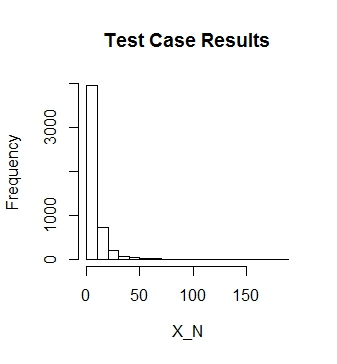
\includegraphics[width=5.5cm]{img/MilTestCase}
\end{center}

\begin{tabular}{cccccc}
    Min. & 1st Qu. &  Median  &   Mean & 3rd Qu.  &   Max.\\ 
  0.1718  & 2.3600 &  4.6110 &  7.4560 &  8.8240 & 187.9000
\end{tabular}
 

\end{frame}

